% You should title the file with a .tex extension (hw1.tex, for example)
\documentclass[11pt]{article}

\usepackage{amsmath}
\usepackage{mathtools}
\usepackage{amssymb}
\usepackage{wrapfig}
\usepackage{fancyhdr}
\usepackage{tikz-qtree}
\usepackage{tikz-qtree-compat}
\usepackage[normalem]{ulem}
\usepackage{tikz}
\usepackage{graphicx}
\DeclareMathOperator*{\argmin}{argmin}
\DeclareMathOperator*{\argmax}{argmax}

\oddsidemargin0cm
\topmargin-2cm     %I recommend adding these three lines to increase the 
\textwidth16.5cm   %amount of usable space on the page (and save trees)
\textheight23.5cm  

\newcommand{\question}[2] {\vspace{.25in} \hrule\vspace{0.5em}
\noindent{\bf #1: #2} \vspace{0.5em}
\hrule \vspace{.10in}}
\renewcommand{\part}[1] {\vspace{.10in} {\bf (#1)}}
\linespread{1.5}

\newcommand{\myname}{Anonymous Authors}
\newcommand{\myhwnum}{12}

\setlength{\parindent}{0pt}
\setlength{\parskip}{5pt plus 1pt}
 
\DeclarePairedDelimiter\abs{\lvert}{\rvert}%

\pagestyle{fancyplain}

\begin{document}

\medskip                        % Skip a "medium" amount of space
                                % (latex determines what medium is)
                                % Also try: \bigskip, \littleskip

\thispagestyle{plain}
{\Large Statistical inference in theoretical models of cognition} \\
Sean R. Bittner, \textit{the DSN alliance}, John P. Cunningham

\section{Figures}
\clearpage

\begin{figure}
\begin{center}
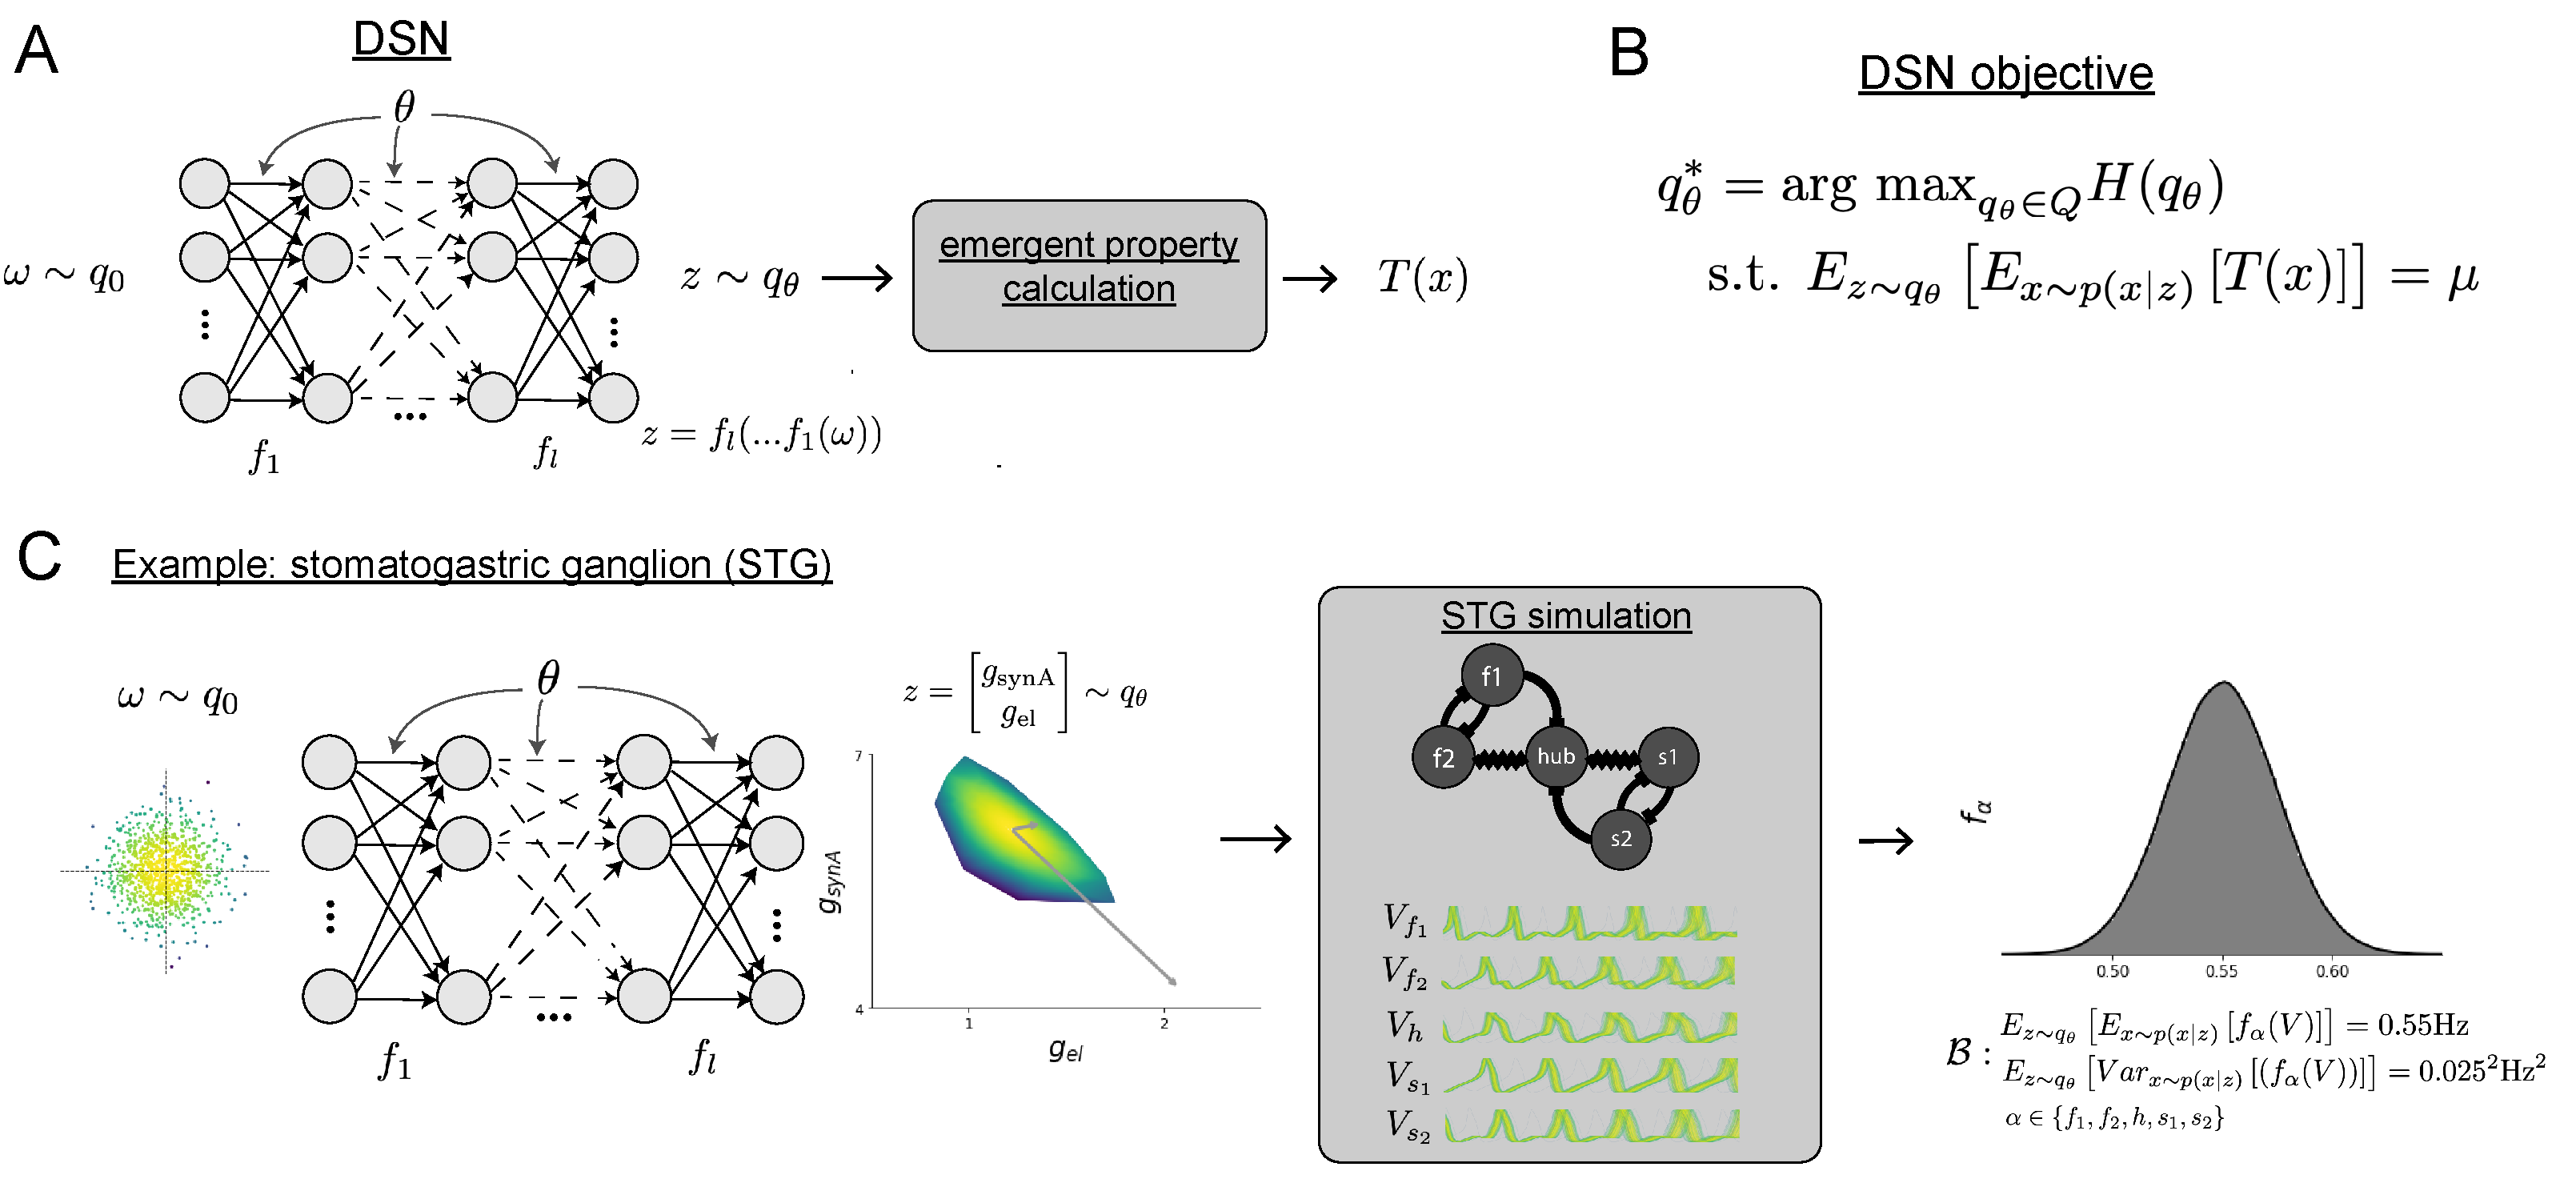
\includegraphics[scale=0.3]{figs/Fig1.pdf}
\end{center}
\caption{}
\end{figure}

\clearpage

\begin{figure}
\begin{center}
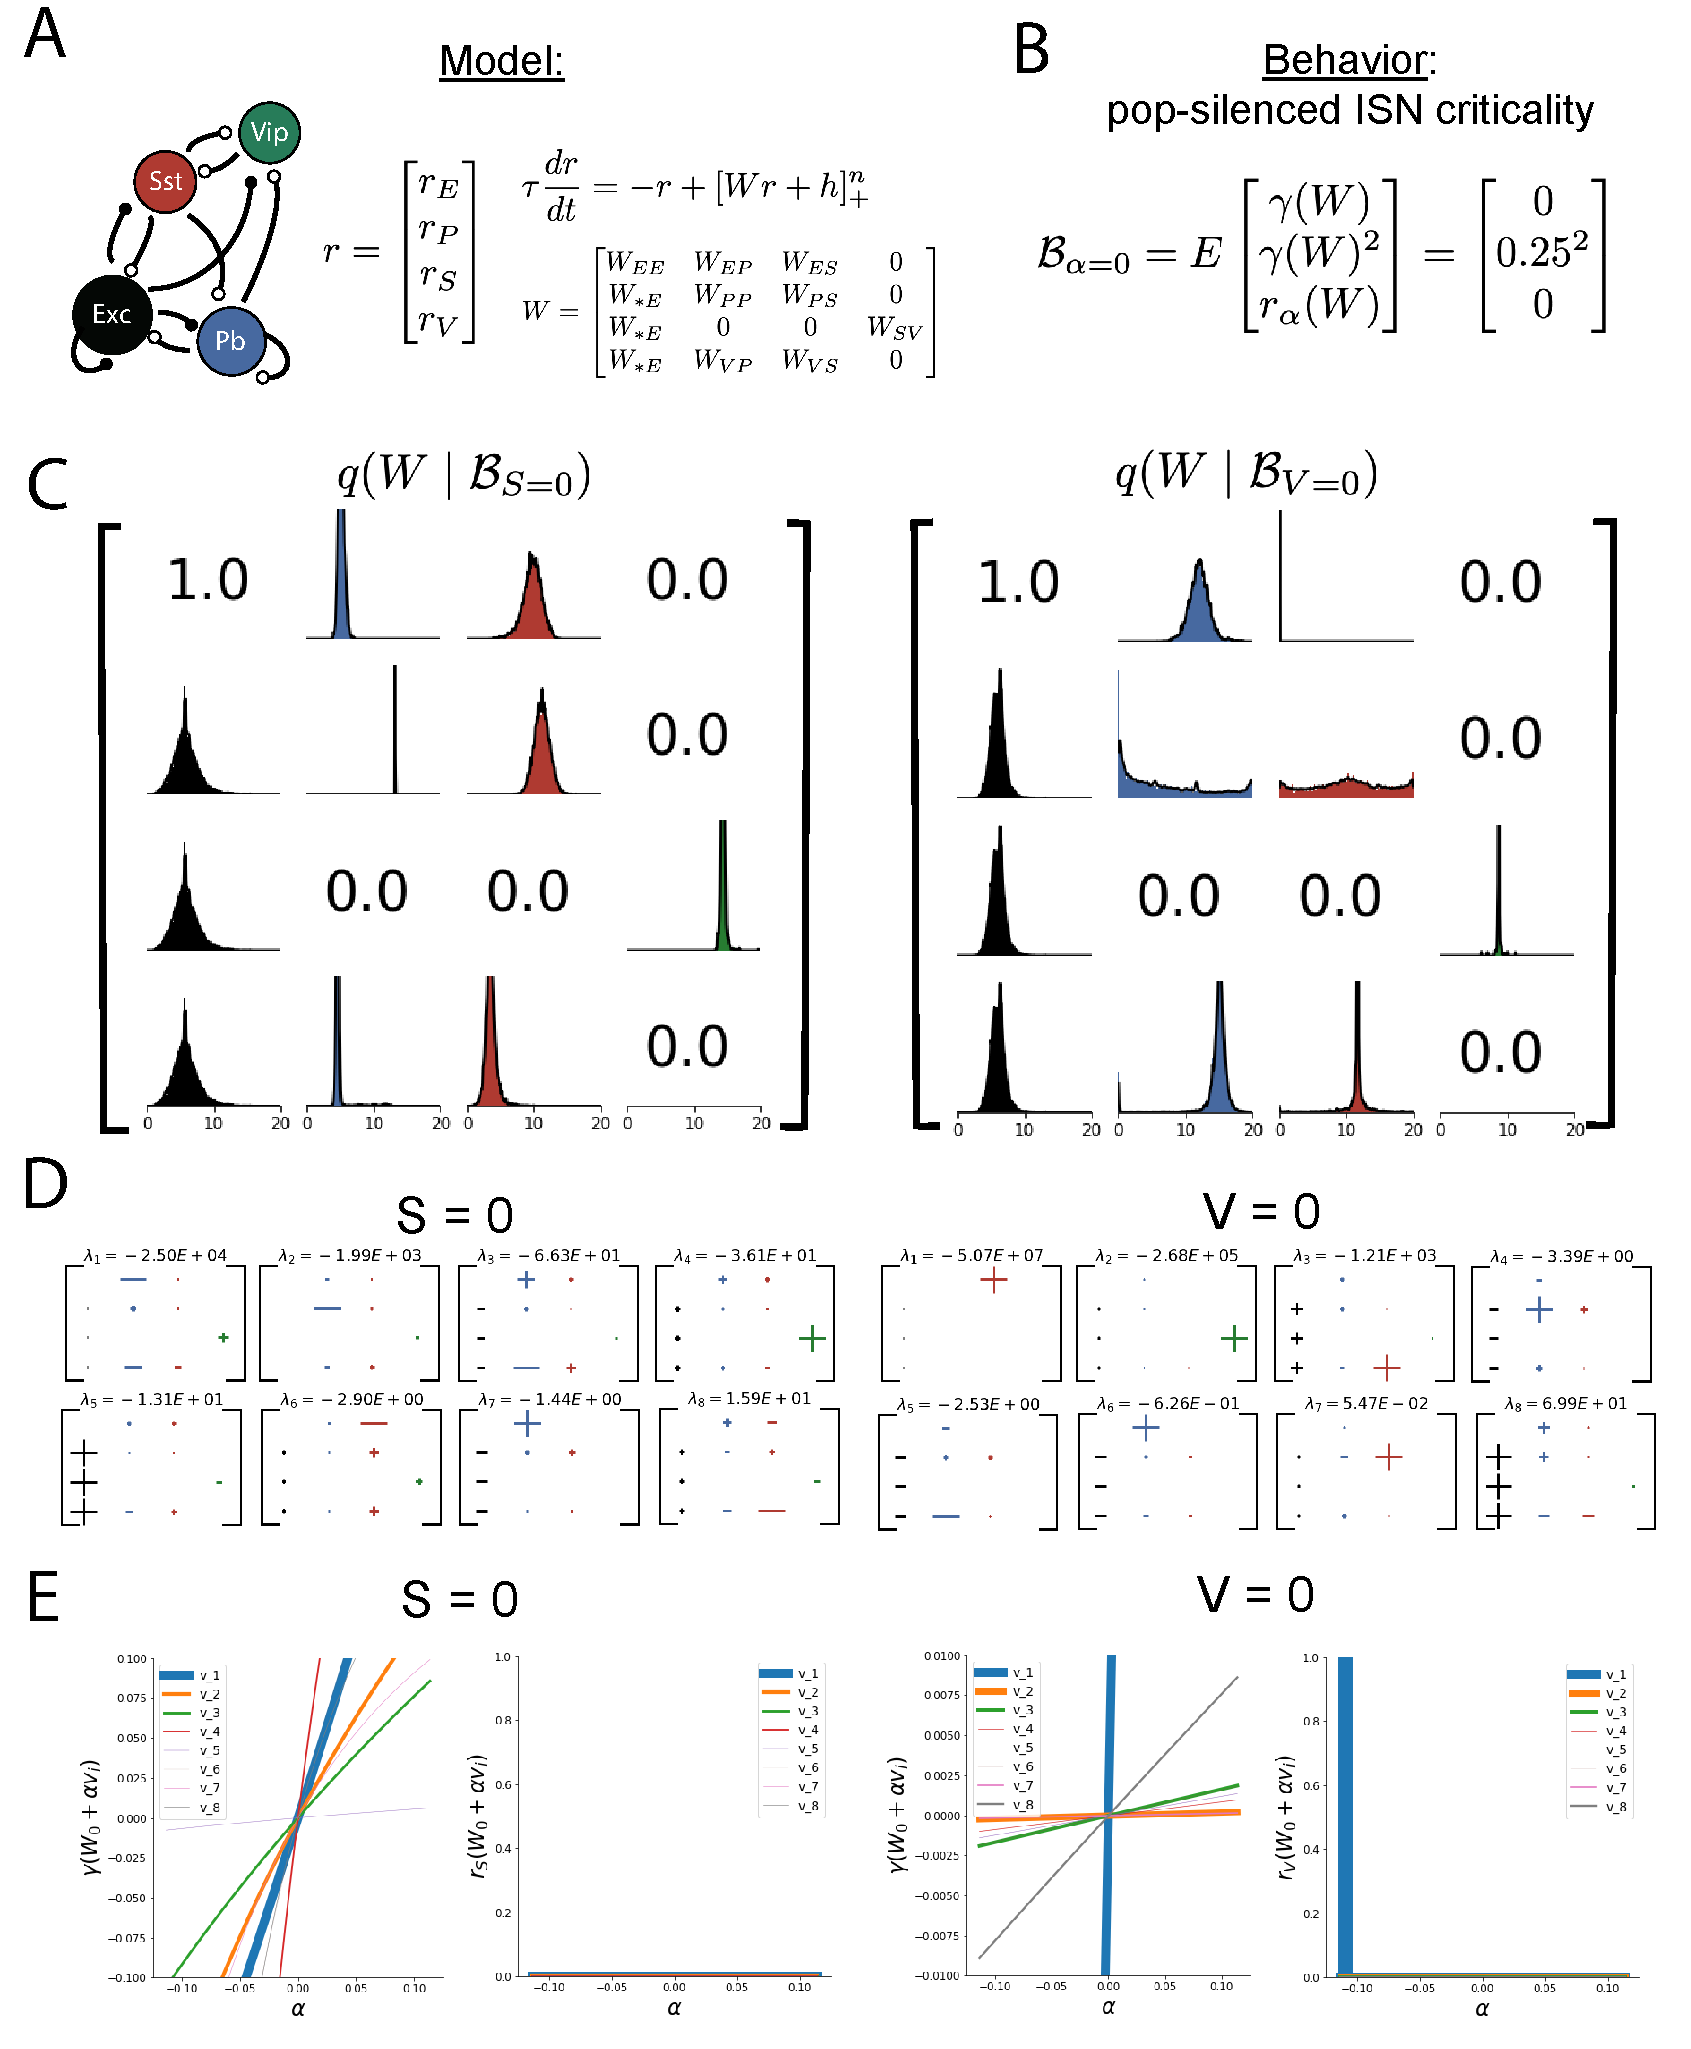
\includegraphics[scale=0.5]{models/V1/V1_Fig/V1_Fig.pdf}
\end{center}
\caption{\protectA.) Model of primary visual cortex (V1) Neurons: E (black), P (blue), S (red), and V (green).  Parameters: weights of the dynamics matrix $W$.  B.) The DSNs are conditioned on population-silenced ISN criticality.  C.) DSN distribution of the parameters of the V1 model conditioned on population-silened ISN criticality.  D.) Eigenmodes of the hessian of each DSN ordered by eigenvalue.  E. Input to silenced population across ISN regimes of the DSN posterior.
}
\end{figure}

\clearpage

\begin{figure}
\begin{center}
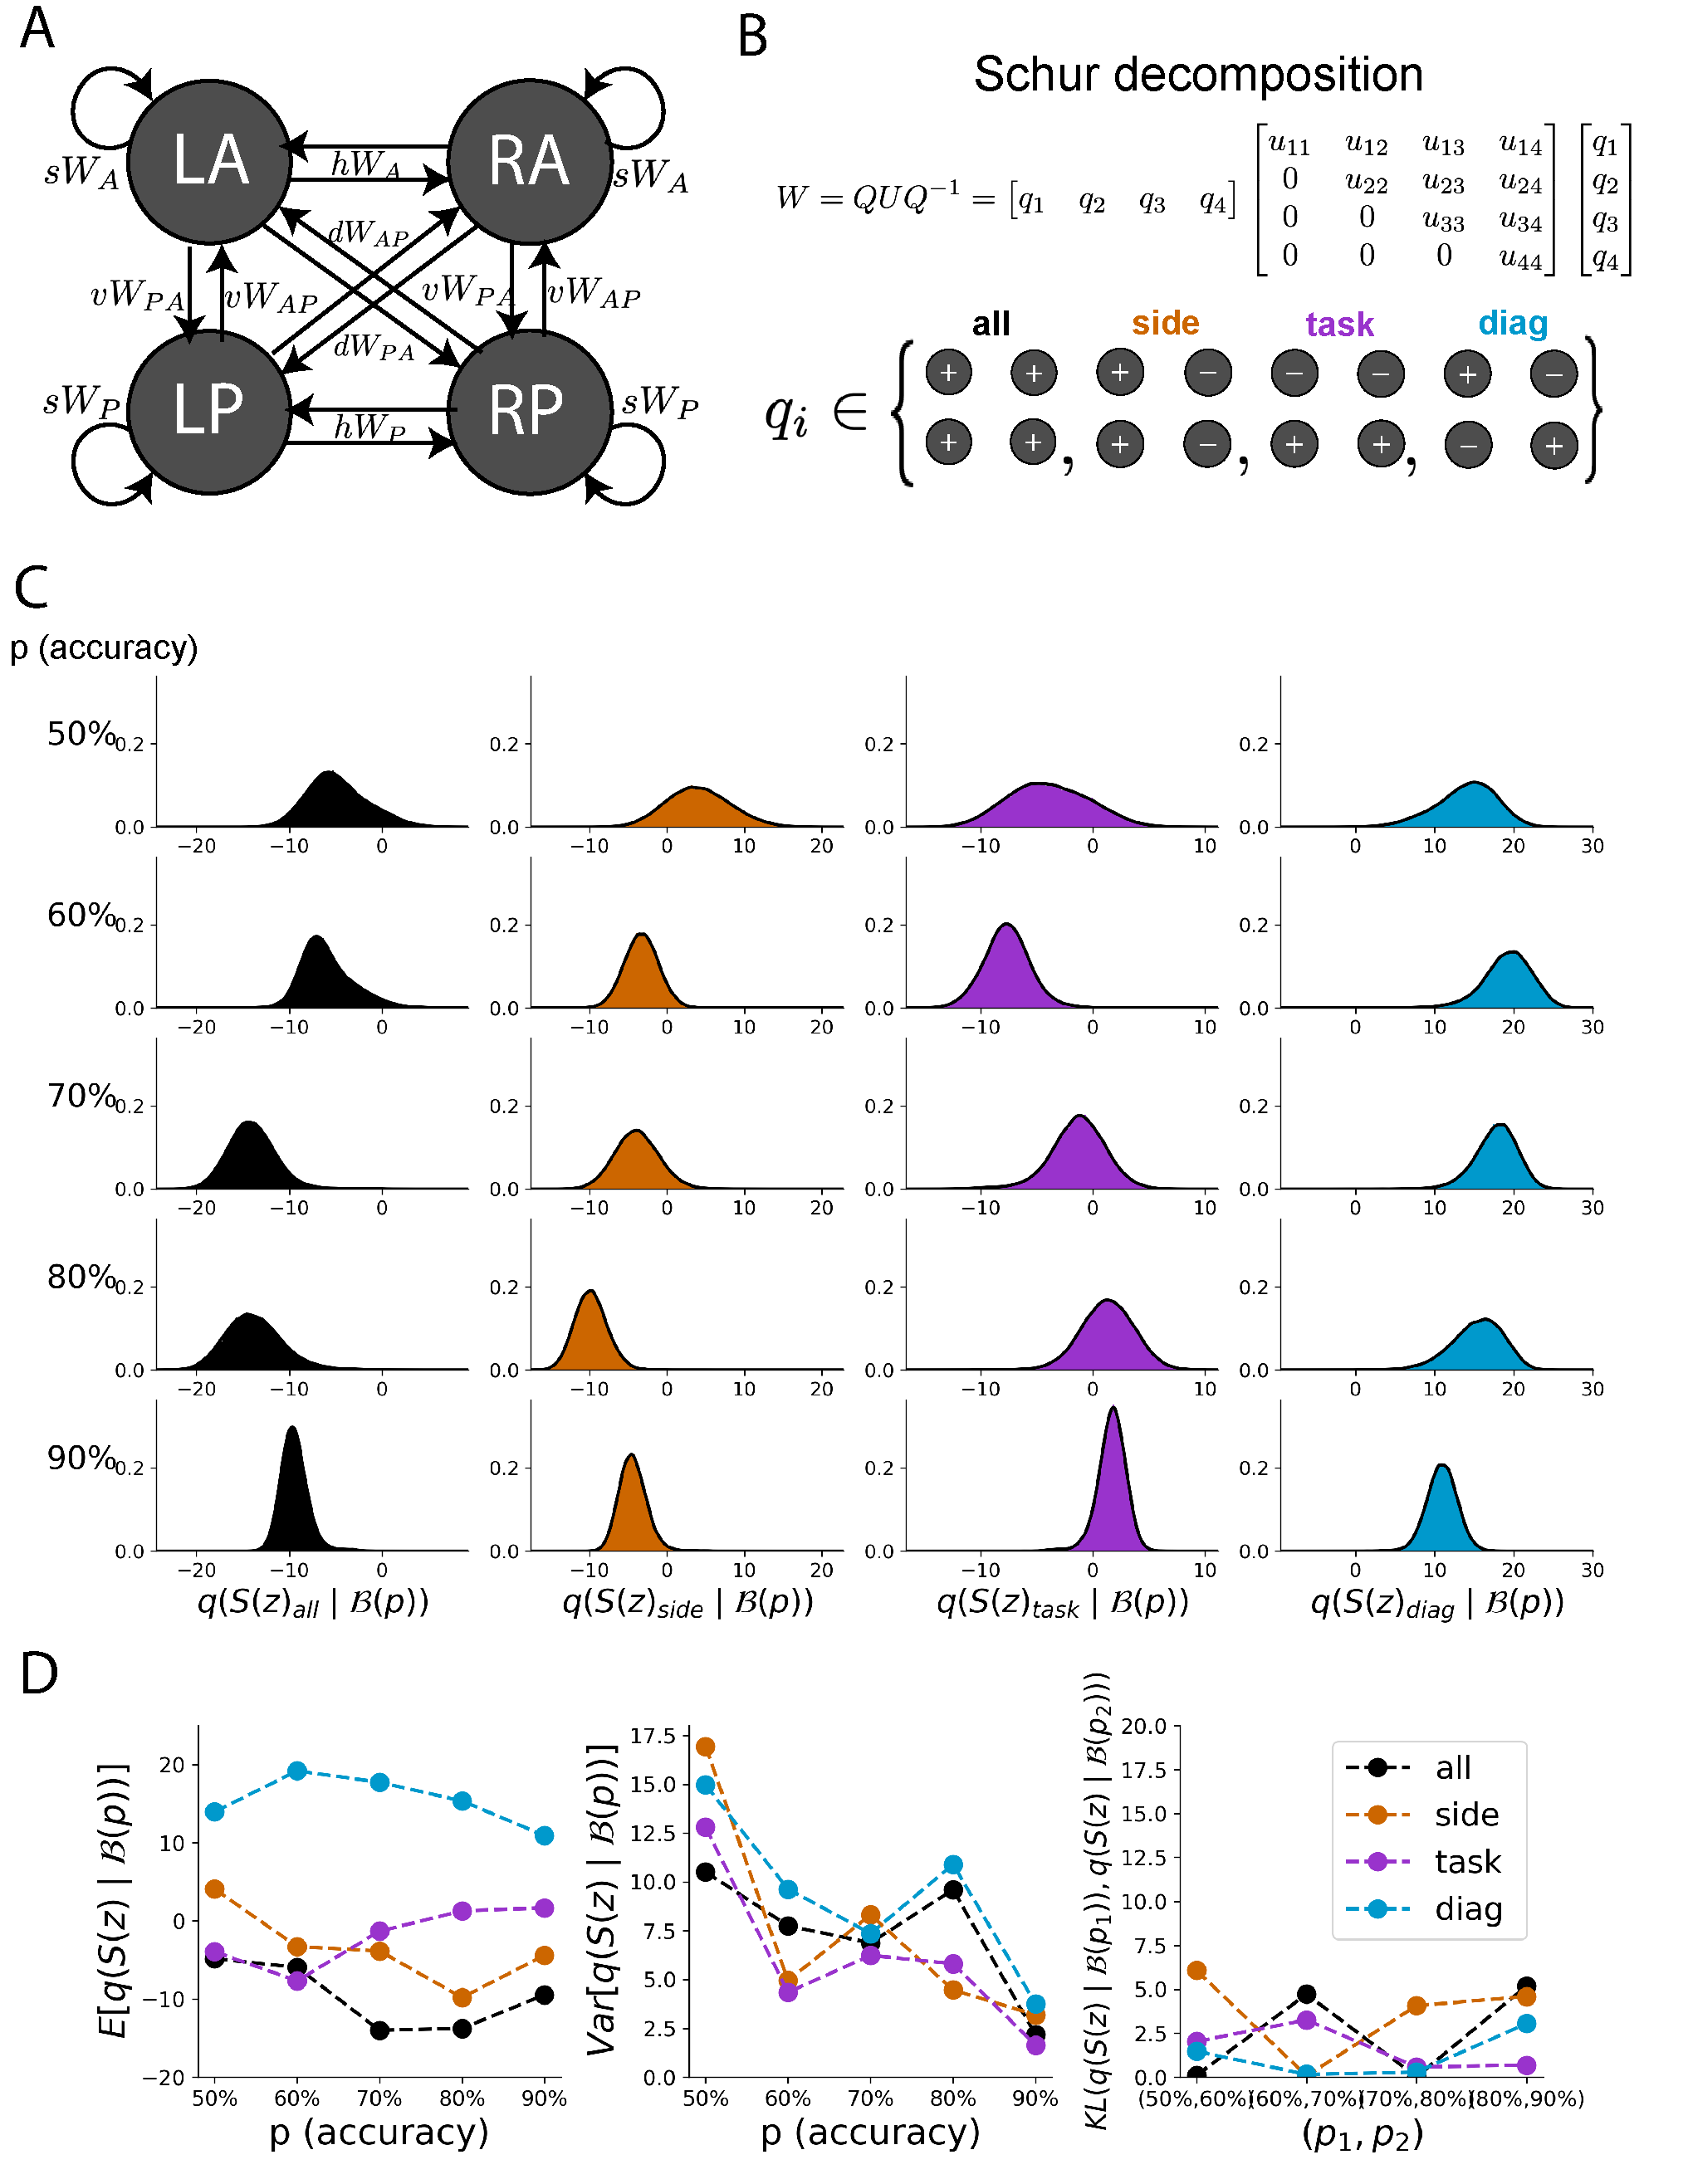
\includegraphics[scale=0.5]{models/SC/SC_Fig/SC_Fig.pdf}
\end{center}
\caption{\protectA.) Model of superior collicullus (SC). Neurons: LP - left pro, RP - right pro, LA - left anti, RA - right anti.  Parameters: sW - self, hW - horizontal, vW -vertical, dW - diagonal weights.  B.) Schur decomposition of W.  C.) DSN distribution of schur mode eigenvalues $S(z)$ with task learning.  D.) DSN means and variances (left and center, respectively) and step-wise KLs.}
\end{figure}
\end{document}

